\section{Zielsetzung}
In diesem Versuch soll die Dichte, Rauigkeit und Schichtdicke eines Polysterolschicht
mithilfe der Röntgenreflektrometrie bestimmt werden.

\section{Theorie}

\subsection{Erzeugung von Röntgenstrahlung}
Elektromagnetische Wellen, die in einem Wellenlängenbereich von ungefähr $10^{-9}\,\unit{\meter}$ bis $10^{-11}\,\unit{\meter}$
liegen, werden als Röntgenstrahlen bezeichnet. Sie haben entsprechend eine Energie von ca. $100\,\unit{\electronvolt}$ bis $250\,\unit{\kilo\electronvolt}$.
Die Röntgenstrahlung im Versuch wird in einer Röntgenröhre erzeugt.

\begin{figure}[H]
  \centering
  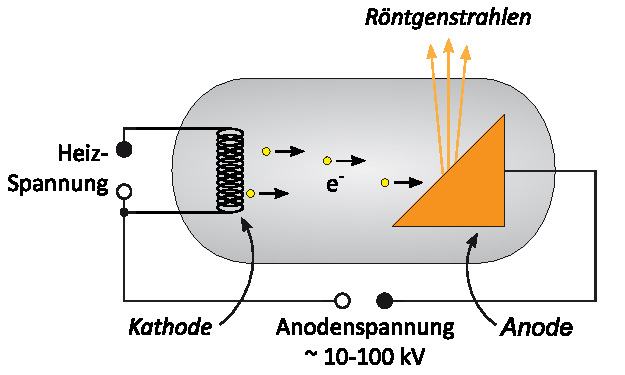
\includegraphics[scale=0.75]{röntgenröhre.pdf}
  \caption{Erzeugung von Röntgenstrahlung in einer Röntgenröhre \cite{uni_goettingen}.}
  \label{fig:roentgenroehre}
\end{figure}
\noindent
Zuerst wird durch das Erhitzen der Glühkathode ($10\,\unit{\kilo\volt}-100\,\unit{\kilo\volt}$) Elektronen freigesetzt (glühelektrischer Effekt).
Die Erzeugung von Röntgenstrahlung in einer Röntgenröhre basiert prinzipiell auf der Beschleunigung von Elektronen 
von der Glühkathode zur Anode. Wenn die Elektronen auf die Anode treffen, entstehen Bremsstrahlung 
und charakteristische Röntgenstrahlung. Die Bremsstrahlung resultiert aus der Abbremsung der Elektronen 
durch das Coulombfeld der Atomkerne, während die charakteristische Röntgenstrahlung durch den Übergang der Elektronen in den 
Atomhüllen erzeugt wird. In Abbildung \ref{fig:roentgenroehre} ist der schematische Aufbau einer 
Röntgenröhre zu sehen.




\subsection{Röntgenstrahlung an einer Grenzfläche}
In Abbildung \ref{fig:reflection_transmission} wird ein Strahl an einer Grenzfläche reflektiert und transmittiert. Dabei 
wird der Einfalls-, bzw. Ausfallswinkels als $\phi$ bezeichnet und $\varphi$ ist der Winkel zwischen der transmittierten Welle und der Grenzebene.
Im Folgenden wird $\phi$ durch $\alpha$ ersetzt und $\varphi$ durch $\alpha\idx{t}$. Eine Unterscheidung zwischen dem Ein- und Ausfallswinkel ist 
nicht zwingend nötig, da diese nach dem Reflektionsgesetz identisch sind.
\begin{figure}[H]
  \centering
  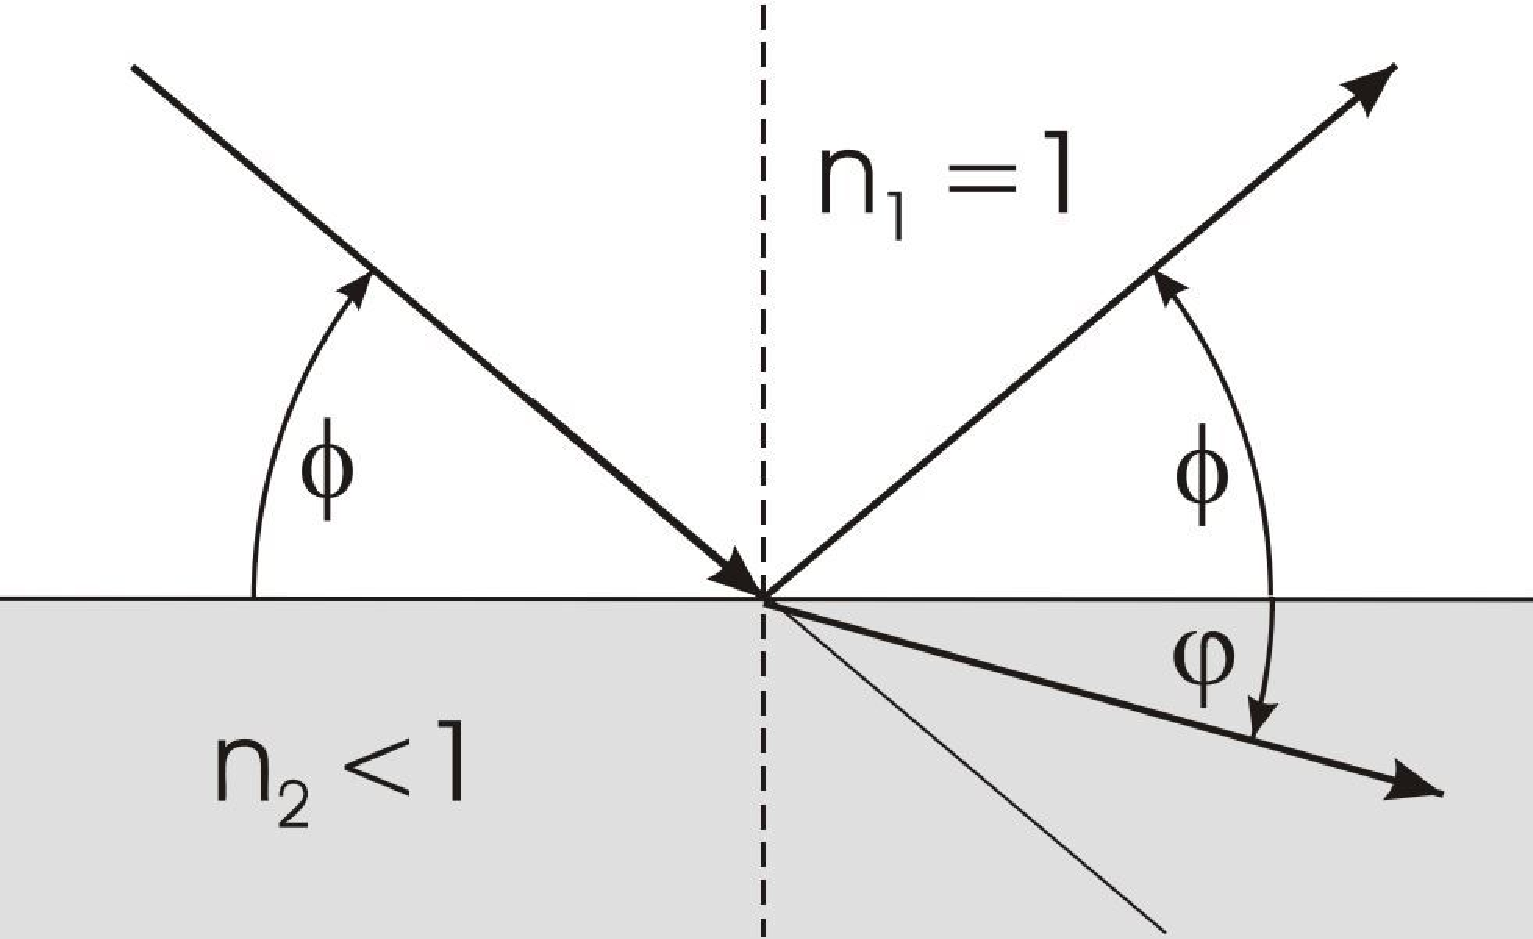
\includegraphics[scale=0.25]{rt.pdf}
  \caption{Lichtstrahl wird an einer Oberfläche reflektiert und transmittiert \cite{uni_giessen}.}
  \label{fig:reflection_transmission}
\end{figure} 
\noindent
Der Brechungsindex beschreibt die Stärke der Brechung von Licht
beim Übergang von einem Medium in ein anderes. Die Lichtgeschwindigkeit im Vakuum
ist eine feste Größe, jedoch ist die Geschwindigkeit in Materie materialspezifisch. Der
Brechungsindex gibt das Verhältnis zwischen der Lichtgeschwindigkeit in Materie und
der Lichtgeschwindigkeit im Vakuum an.
In Falle von Röntgenstrahlung ist der Brechungsindex
\begin{equation}
  n= 1 - \delta + i \beta , 
\end{equation}
wobei $\beta$ und $\delta$ die materialspezifische Absorptionkonstante und Dispersion (Größenordnung $10^{-6}$) sind.
Ab einem kritischen Winkel $\alpha\idx{C}$ tritt Totalreflexion auf. Diese ist 
\begin{equation}
  \alpha\idx{C} \approx \sqrt{2 \delta} = \lambda \sqrt{\frac{\rho r\idx{e}}{\pi}}
  \label{eq:kritisch}
\end{equation}
unter der Annahme von kleinen Winkeln. Hier ist $\lambda$ die Wellenlänge, $\rho$ die Elektronendichte des Stoffes und 
$r\idx{e}$ der Elektronenradius.
Um das Amplitudenverhältnis des reflektierten und transmittierten Anteil des Lichts, wenn es auf eine Grenzfläche zwischen zwei 
verschiedene optische Medien trifft, zu beschreiben, 
werden Fresnelgleichungen herangezogen. Dabei wird zwischen senkrecht (s) und parallel (p) polarisiertes Licht unterschieden.
Bei Röntgenstrahlung können die Polarisationseigenschaften jedoch vernachlässigt werden, da sie unpolarisiert sind und keine bevorzugte 
Ausrichtung besitzen. So kann bei Betrachtung von Röntgenstrahlung angenommen werden, dass beide Polarisationsanteile ungefähr gleich sind.
Für den Reflektions-, bzw. Transmissionskoeffizient gilt
\begin{equation}
  r= \frac{n\idx{1} \sin \alpha\idx{i} - n\idx{2} \sin \alpha\idx{t}}{n\idx{1} \sin \alpha\idx{i} + n\idx{2} \sin \alpha\idx{t}}
\end{equation}
und
\begin{equation}
  t= \frac{2n\idx{1} \sin \alpha\idx{i}}{{n\idx{1} \sin \alpha\idx{i} + n\idx{2} \sin \alpha\idx{t}}}.
\end{equation}
Hierbei stehen $n\idx{1}$ und $n\idx{2}$ für die Brechungsindizes des ersten, bzw. zweiten Mediums.
Die Intensität des Lichtstrahls ist proportional zum Quadrat der Feldstärke. Die Reflektivität ist das Verhältnis 
zwischen der reflektierten Strahlintensität $I\idx{r}$ und der einfallenden Strahlintensität $I\idx{e}$ und wird durch 
\begin{equation*}
  R = \frac{I\idx{r}}{I\idx{e}} =|r|^2 
\end{equation*}
ausgedrückt.




\subsection{Reale Proben}
Bisher wurde in der Reflexionsbetrachtung von ideal glatten Grenzflächen und einschichtigen Proben ausgegangen. Allerdings trifft diese Annahme 
nicht auf reale Grenzflächen zu. Die Eigenschaften realer Proben werden in folgende Abschnitte behandelt.

\subsubsection{Mehrschichtsysteme}
In diesem Abschnitt werden Mehrschichtsysteme behandelt. In Abbildung \ref{fig:reflectivity} ist
Reflektivit eines Siliziumwafers mit einem Polysterolschicht bei einer Wellenlänge von $\lambda = 1,54\,\unit{\angstrom}$ dargestellt. 
In dem Subplot wird ein Bereich vergrößert und die kritischen Winkel $\alpha\idx{C}$ jeweils für den Siliziumwafer und die Polysterolschicht gekennzeichnet.
Für ein Einfallswinkel $\alpha\idx{i} > \alpha\idx{C}$ findet keine Totalreflexion mehr statt, so dass die Reflektivität danach drastisch abnimmt.
\begin{figure}[H]
  \centering
  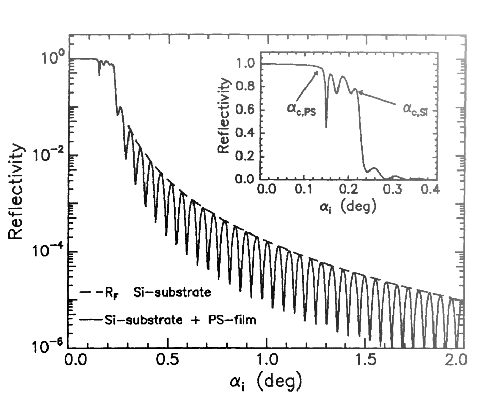
\includegraphics[scale=1.2]{reflectivity_plot.pdf}
  \caption{Reflektivit eines Siliziumwafers mit einem Polysterolschicht anhängig vom Einfallswinkel der Strahlung \cite{tolan}.}
  \label{fig:reflectivity}
\end{figure}
\noindent
Zudem sind Oszillationen zu erkennen, die aufgrund von Interferenzeffekte an den Grenzflächen der beiden Schichten auftreten.
Diese werden auch als Kiessig-Oszillationen bezeichnet. Sie entstehen, indem ein Teil der Strahlung, der das erste Medium durchdringt, 
an der Grenzfläche zum zweiten Medium reflektiert wird. Dieser reflektierte Anteil interferiert dann mit dem Teil der Strahlung, der 
bereits am ersten Medium reflektiert wurde. Über die Gleichung 
\begin{equation}
d = \frac{\lambda}{2\upDelta \alpha\idx{i}}
\label{eq:schicht}
\end{equation}
kann die Schichtdicke berechnet werden. Dabei ist $\upDelta \alpha\idx{i}$ der Abstand zwischen zwei Minima/Maxima.
Bestehen Systeme aus mehr als zwei Schichten, überlagern sich die Oszillationen. Um diese Überlagerung zu quantifizieren, wird der 
Parratt-Algorithmus verwendet. Dieser ist ein rekursives Verfahren zur Beschreibung eines Mehrschichtsystems. 
In Abbildung \ref{fig:multischichtsystem} ist ein solches mit $N$-Schichten abgebildet. Die Welle wird an jeder Grenzfläche zum Teil 
reflektiert (blau) und transmittiert (rot). $T\idx{j}$ und $R\idx{j}$ sind dabei die Amplituden für den transmittierten, bzw. reflektierten 
Strahl.
\begin{figure}[H]
  \centering
  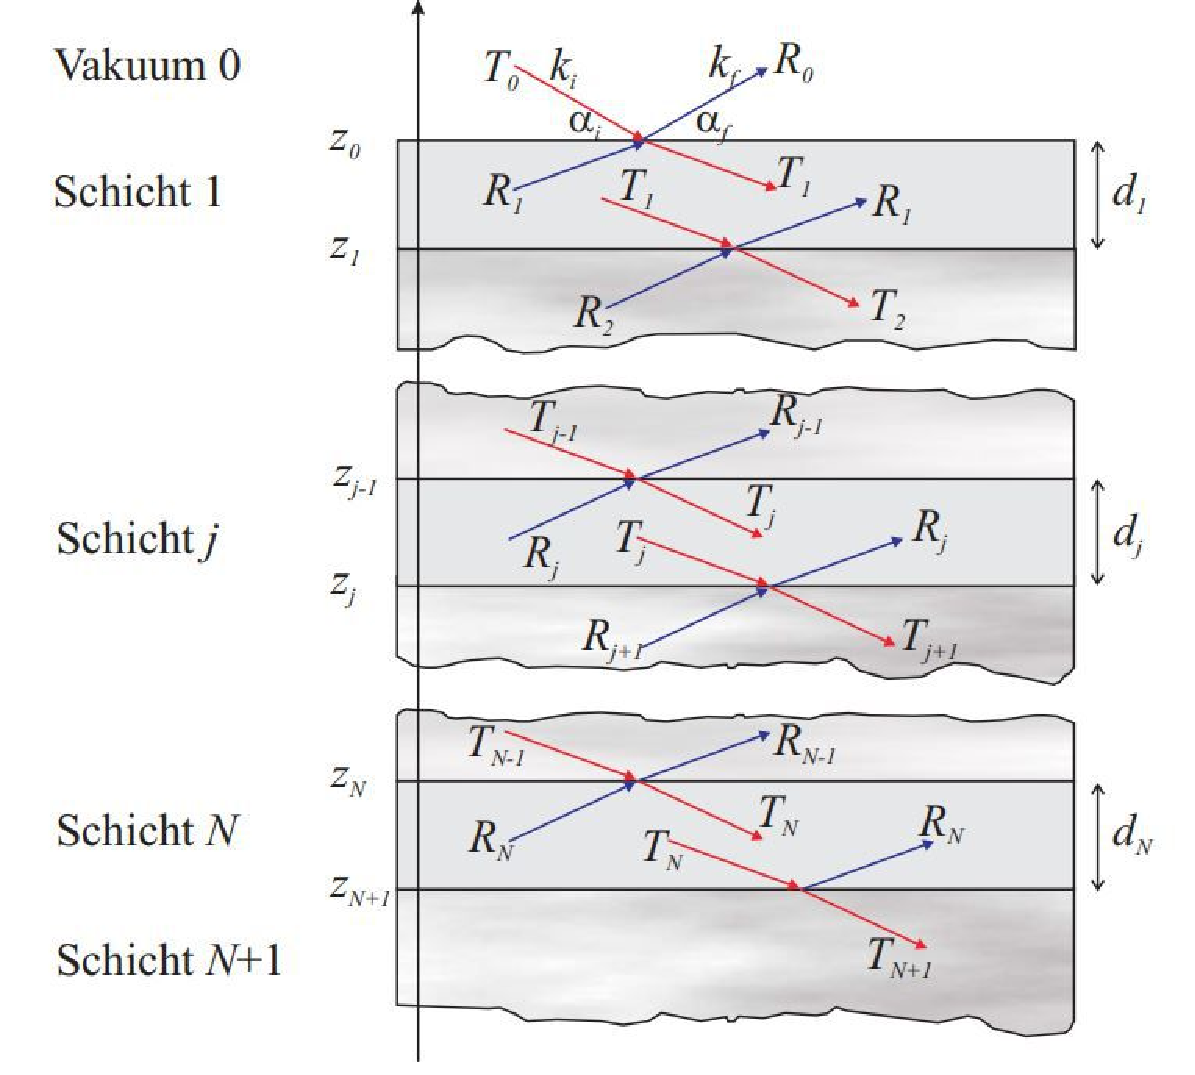
\includegraphics[scale=0.4]{mehrschichtsystem.pdf}
  \caption{Reflexion und Brechung an einem Mehrschichtsystem mit $N$ Grenzschichten \cite{Bachelorarbeit_Bertram}.}
  \label{fig:multischichtsystem}
\end{figure}
\noindent
Der Parratt-Algorithmus durchläuft rekursiv alle Schichten, beginnend mit der untersten Schicht (Schicht $N$). 
Es wird angenommen, dass die Dicke der darunter liegenden Schicht deutlich größer als die Tiefe ist, auf die Röntgenstrahlen 
in ein Material eindringen können. Daraus folgt die Bedingung $R\idx{N,N+1}=0$. Die Welle wird nämlich an der letzten 
Grenzfläche transmittiert (und reflektiert), jedoch nicht wieder von einer weiteren Schicht zurückreflektiert. 
Ausgehend von der untersten Schicht kann jeweils das Verhältnis zwischen $T\idx{j}$ und $R\idx{j}$ 
mit 
\begin{equation}
  X\idx{j} = \frac{R\idx{j}}{T\idx{j}} = \frac{r\idx{j,j+1} + X\idx{j+1} \exp({2ik\idx{j+1,z}d\idx{j}})}{1+ r\idx{j,j+1} X\idx{j+1} \exp({2ik\idx{j+1,z}d\idx{j}})} \exp({-2ik\idx{j,z}d\idx{j}})
\end{equation}
ermittelt werden. Hierbei ist $d\idx{j}$ die Dicke der $j$-ten Schicht und 
\begin{equation}
  r\idx{j,j+1} = \frac{k\idx{k,z} - k\idx{j+1,z}}{k\idx{k,z} + k\idx{j+1,z}}
\end{equation}
der Fresnel-Koeffizient für die Schichten $j$ und $j+1$ und 
\begin{equation}
  k\idx{z,j} = k \sqrt{n^2\idx{j}-\cos^2\alpha\idx{i}}
\end{equation}
die $z$-Komponente des $j$-ten Wellenvektors.


\subsubsection{Rauigkeit}
Reale Proben haben keine ideal glatte Grenzflächen, was jedoch bis jetzt in der Theorie angenommen wurde. 
Um dies zu korrigieren, werden die Fresnel-Koeffizienten modifiziert
\begin{equation}
  \tilde{r}\idx{j+1,j} = r\idx{j,j+1} \exp(-2k\idx{z,j}k\idx{z,j+1} \sigma^2\idx{j})
\end{equation}
und
\begin{equation}
  \tilde{t}\idx{j+1,j} = t\idx{j,j+1} \exp \left ((k\idx{z,j}-k\idx{z,j+1})^2 \frac{\sigma^2\idx{j}}{2} \right ),
\end{equation}
wobei $\sigma$ für die Rauigkeit steht. Wird $\sigma=0$ eingesetzt, so resultierten wieder die vorherigen Fresnel-Koeffizienten
für ideal glatte Ebenen. Des Weiteren wird angenommen, dass $\sigma << d$ ist.
Das Auswerten mit dem Parratt-Algorithmus erfolgt mit diesen angepassten Fresnel-Koeffizienten.







\subsection{Korrektur Geometriefaktor}
Der Röntgenstrahl trifft auf die Probenoberfläche und erst ab einem bestimmten Geometriewinkel
\begin{equation*}
  \alpha\idx{G} = \mathrm{arcsin} \left ( \frac{d\idx{0}}{D} \right )
\end{equation*}
findet die vollständige Reflexion des Strahls statt. Bei sehr geringen Winkeln wird der Strahl nicht vollständige reflektiert.
Zusätzliche Bedingungen hinsichtlich des Einfallswinkels sind erforderlich, um weitere Berechnungen durchzuführen.
Der sogenannte Geometriefaktor wird eingeführt und ist als
\begin{equation*}
  G = 
\begin{cases}
1 & \alpha\idx{i} \geq \alpha\idx{G} \\
\frac{D \sin \alpha\idx{i}}{d\idx{0}} & \, \alpha\idx{i} < \alpha\idx{G}, \\
\end{cases}
\end{equation*}
gegeben. Dabei entspricht $D$ die Länge der Probe, $d\idx{0}$ die gesamte Strahlbreite und $D \sin \alpha\idx{i}$ damit die 
effektive Strahlbreite.